
\documentclass[11pt,a4paper]{article}
\usepackage[utf8]{inputenc}
\usepackage[T1]{fontenc}
\usepackage[english]{babel}
\usepackage[a4paper,margin=2.2cm]{geometry}
\usepackage{lmodern}
\usepackage{microtype}
\usepackage{xcolor}
\usepackage{graphicx}
\usepackage{float}
\usepackage{booktabs}
\usepackage{longtable}
\usepackage{tabularx}
\usepackage{array}
\usepackage{multirow}
\usepackage{amsmath,amssymb}
\usepackage{enumitem}
\usepackage{hyperref}
\usepackage{caption}
\usepackage{fancyhdr}
\usepackage{titlesec}
\usepackage[most]{tcolorbox}
\usepackage{lastpage}
\usepackage{setspace}
\usepackage{url}
\usepackage{tikz}
\usepackage{pgfplots}
\usepackage{siunitx}
\pgfplotsset{compat=1.18}
\usetikzlibrary{positioning,arrows.meta,shapes.geometric,fit}

\hypersetup{colorlinks=true,linkcolor=blue!50!black,citecolor=blue!50!black,urlcolor=blue!60!black,pdftitle={StarCraft II Outcome Prediction: Final Reproducible Paper v6.2},pdfauthor={OpenAI}}

\definecolor{accent}{RGB}{28,56,110}
\definecolor{softblue}{RGB}{242,246,252}
\definecolor{softgray}{RGB}{246,246,246}
\definecolor{softwarn}{RGB}{255,249,235}
\definecolor{softgreen}{RGB}{240,248,242}
\definecolor{linegray}{RGB}{210,215,225}

\pagestyle{fancy}
\fancyhf{}
\fancyhead[L]{StarCraft II Outcome Prediction}
\fancyhead[R]{Final project paper v6.2}
\fancyfoot[C]{\thepage/\pageref{LastPage}}
\setlength{\headheight}{14pt}

\titleformat{\section}{\large\bfseries\color{accent}}{\thesection}{0.7em}{}
\titleformat{\subsection}{\normalsize\bfseries\color{accent}}{\thesubsection}{0.6em}{}
\titleformat{\subsubsection}{\normalsize\bfseries}{\thesubsubsection}{0.5em}{}
\setlist[itemize]{topsep=3pt,itemsep=2pt,leftmargin=1.3em}
\setlist[enumerate]{topsep=3pt,itemsep=2pt,leftmargin=1.5em}
\setstretch{1.08}
\setlength{\parindent}{0pt}
\setlength{\parskip}{0.55em}

\newtcolorbox{keybox}{colback=softblue,colframe=accent!55!black,boxrule=0.6pt,arc=2mm,left=2mm,right=2mm,top=1.4mm,bottom=1.4mm}
\newtcolorbox{resultbox}{colback=softgreen,colframe=green!40!black,boxrule=0.6pt,arc=2mm,left=2mm,right=2mm,top=1.4mm,bottom=1.4mm}
\newtcolorbox{warningbox}{colback=softwarn,colframe=orange!55!black,boxrule=0.6pt,arc=2mm,left=2mm,right=2mm,top=1.4mm,bottom=1.4mm}

\newcolumntype{Y}{>{\raggedright\arraybackslash}X}

\begin{document}

\begin{titlepage}
\centering
\vspace*{1.9cm}
{\Large Machine Learning Project\par}
\vspace{0.45cm}
{\Huge\bfseries StarCraft II Outcome Prediction\par}
\vspace{0.3cm}
{\Large A full reproducible study from replay-derived dataset construction to calibrated final model selection\par}
\vspace{1.1cm}
\begin{tcolorbox}[width=0.92\textwidth,colback=softblue,colframe=accent,arc=2mm,boxrule=0.8pt]
This paper presents the final consolidated version of the project as a continuous manuscript. The emphasis is not only on which model performs best, but on how replay files were transformed into a valid supervised-learning dataset, how replay-aware evaluation was enforced, and how staged conclusions were corrected by full multi-seed evidence.
\end{tcolorbox}
\vfill
\small
\begin{tabularx}{0.90\textwidth}{@{}>{\raggedleft\arraybackslash}p{0.24\textwidth} Y@{}}
\textbf{Document type:} & Final project paper, version 6.2 \\
\textbf{Experimental scope:} & Dataset construction, full multi-seed comparison, calibration, and deep challenger \\
\textbf{Dataset variants:} & \texttt{v3\_1\_fixed}, \texttt{v3\_2\_combatfix} \\
\textbf{Final date:} & April 2026 \\
\end{tabularx}
\normalsize
\vfill
\end{titlepage}

\section*{Abstract}
This paper studies match outcome prediction in \emph{StarCraft II} using tabular snapshots extracted from replay files. The project is deliberately framed as a full pipeline problem rather than as a model-only benchmark. The raw replay corpus used for dataset generation consists of 71 replaypacks and 24,057 replays. This corpus is transformed into a time-indexed supervised dataset through a deterministic pipeline that parses raw replay files, aligns per-player state, applies eligibility filtering, emits one row every 15 seconds after an opening exclusion window, and assigns replay-level labels. After the project filters are applied, the final usable replay corpus contains 23,241 replays and yields a tabular dataset of 892,047 rows.

An important contribution of the work is experimental discipline. Because many rows come from the same replay, the evaluation protocol uses replay-aware grouped splits, separates validation from final test usage, and evaluates final claims over three seeds (42, 43, 44). The model comparison ultimately focuses on Random Forest (RF), XGBoost (XGB), and a final deep multilayer perceptron challenger. RF is strongest with the \texttt{no\_counter} profile, while XGB is evaluated on the full feature set.

The final full multi-seed benchmark shows that \texttt{v3\_1\_fixed} is at least as strong as \texttt{v3\_2\_combatfix}. RF and XGB finish nearly tied: RF is marginally stronger on classification-oriented metrics, while XGB is marginally stronger on probability-oriented metrics such as log loss and remains well calibrated without meaningful post-hoc improvement. A final deep challenger is competitive, but does not surpass the tabular finalists. The resulting recommendation therefore depends on the downstream objective: RF + \texttt{v3\_1\_fixed} + \texttt{no\_counter} for classification, and XGB + \texttt{v3\_1\_fixed} + full features for probability quality.

\tableofcontents
\newpage

\section{Introduction}
Predicting the winner of a \emph{StarCraft II} match from replay snapshots is a compelling machine-learning problem because it combines temporal development, partial observability, domain-specific structure, and large-scale tabular prediction. At any time point in a match, the final outcome depends on economic state, army composition, technology, scouting asymmetry, map control, and latent strategic intent. A useful predictor therefore depends not only on model capacity, but on whether the replay has been converted into a representation that preserves strategic signal while remaining comparable across matches.

This project treats outcome prediction as a full data-to-model pipeline. The raw object is not an image, a tensor, or a single summary vector, but a replay archive. The replay must first be transformed into a dataset that exposes the game state through synchronized snapshot rows, and only then does model comparison become meaningful. That framing shaped the entire project: dataset construction, feature engineering, grouped splitting, model selection, calibration, and final evaluation all had to be made reproducible before the final conclusions could be trusted.

Two questions drove the work:
\begin{enumerate}
    \item can replay-derived tabular snapshots predict the final match winner reliably under a replay-aware full-scale protocol?
    \item once the evaluation is disciplined enough, which conclusions actually survive: which dataset variant is strongest, which model family is strongest, and which aspects of probability quality differ from classification quality?
\end{enumerate}

\begin{keybox}
The most important scientific decision in this project is to postpone the final story until the full replay-aware multi-seed evidence is complete. This turns the project from a sequence of promising intermediate experiments into a benchmark with defensible final conclusions.
\end{keybox}

\section{Related Work and Context}
The project sits at the boundary between competitive-game analytics, tabular supervised learning, and partially observed sequential environments. Many game-analysis pipelines attempt to learn from rich state streams, but in practice the modeling choice is inseparable from the representation choice: whether one feeds a learner raw tensors, summary features, or time-indexed observations strongly determines what can be learned.

This work intentionally adopts a tabular snapshot view. That design serves two purposes. First, it creates a large supervised corpus from replay files without requiring raw spatial modeling. Second, it makes replay-aware evaluation and feature-family analysis tractable. In exchange, the work does not claim to solve the full sequential game; instead, it asks which strategic signal remains recoverable from a high-quality tabular state description.

The model families used in the project reflect different hypotheses about the problem:
\begin{itemize}
    \item \textbf{Logistic regression} tests how much signal is already linearly separable.
    \item \textbf{Random Forest} tests whether strong threshold-based ensemble rules over engineered state variables can classify the winner robustly.
    \item \textbf{XGBoost} tests whether boosted trees can improve ranking and probability quality through residual correction and stage-wise fitting.
    \item \textbf{Deep MLP} tests whether a flexible non-linear model can exploit interactions not already captured by tree ensembles.
\end{itemize}

A second contextual lens is partial observability. Even though the final learning problem is supervised, the strategic state of the match is never fully visible from a single snapshot. Hidden tech, imperfect scouting, delayed information, and intention all remain latent. This observation is not incidental: it motivates both the engineered feature design and the POMDP-like appendix in Section~\ref{app:pomdp}.

\section{Dataset Construction}
\subsection{Why dataset construction is a core contribution}
In this project the dataset is not a passive by-product of an existing benchmark. It is constructed through a replay-to-snapshot process that determines what the learning problem even is. The validity of the final conclusions therefore depends directly on whether the dataset:
\begin{itemize}
    \item preserves enough strategic structure from the replay,
    \item avoids leakage across train and test,
    \item keeps rows comparable across different matches,
    \item and supports feature-family analysis rather than only black-box prediction.
\end{itemize}

For this reason, dataset construction is not treated as a short preprocessing note. It is one of the main technical foundations of the paper.

\subsection{Replay-to-snapshot pipeline}
The final corpus is built from replay archives through a deterministic pipeline that converts each replay into multiple time-indexed supervised rows. The high-level structure is shown in Figure~\ref{fig:pipeline}.

\begin{figure}[H]
\centering
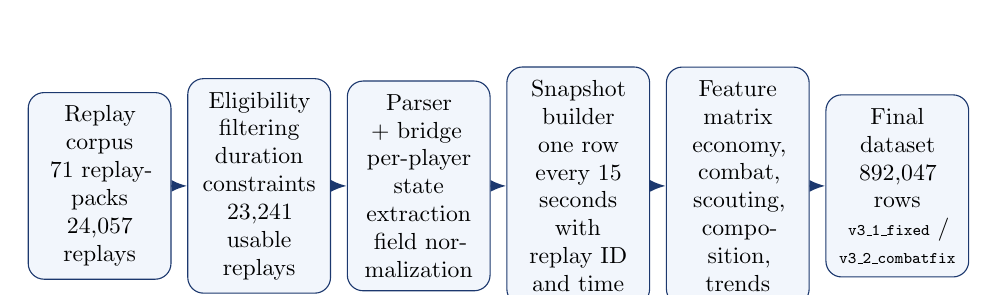
\begin{tikzpicture}[
scale=0.84,
transform shape,
node distance=0.72cm and 0.24cm,
block/.style={draw=accent, rounded corners=2mm, fill=softblue, minimum height=11mm, text width=0.145\textwidth, align=center, inner sep=2.0mm},
arrow/.style={-{Latex[length=2mm]}, thick, draw=accent}
]
\node[block] (r) {Replay corpus\\71 replaypacks\\24,057 replays};
\node[block, right=of r] (e) {Eligibility filtering\\duration constraints\\23,241 usable replays};
\node[block, right=of e] (p) {Parser + bridge\\per-player state extraction\\field normalization};
\node[block, right=of p] (s) {Snapshot builder\\one row every 15 seconds\\with replay ID and time};
\node[block, right=of s] (f) {Feature matrix\\economy, combat, scouting, composition, trends};
\node[block, right=of f] (v) {Final dataset\\892,047 rows\\{\scriptsize\texttt{v3\_1\_fixed}} / {\scriptsize\texttt{v3\_2\_combatfix}}};
\draw[arrow] (r) -- (e);
\draw[arrow] (e) -- (p);
\draw[arrow] (p) -- (s);
\draw[arrow] (s) -- (f);
\draw[arrow] (f) -- (v);
\end{tikzpicture}
\caption{Deterministic replay-to-snapshot pipeline used to build the final supervised dataset, from the raw replay corpus to the filtered replay set and final tabular rows.}
\label{fig:pipeline}
\end{figure}

The stages are:
\begin{enumerate}
    \item \textbf{Replay corpus and eligibility filtering.} The raw project corpus contains 71 replaypacks and 24,057 replays. Before snapshot generation, the pipeline applies project eligibility rules, most importantly the match-duration constraints required by fixed-interval snapshot extraction, yielding 23,241 usable replays.
    \item \textbf{Parser and bridge normalization.} Parser and bridge layers normalize field names, align both players into a common row structure, and expose stable variables suitable for feature engineering.
    \item \textbf{Snapshot emission.} The builder emits one row every 15 seconds after the opening exclusion window.
    \item \textbf{Feature generation.} Economy, combat, scouting, composition, and temporal features are assembled into the final tabular observation.
    \item \textbf{Label assignment.} Each row inherits the final replay winner via the binary target \texttt{p1\_wins}, while preserving the grouping key \texttt{replay\_id} and the temporal coordinate \texttt{time\_sec}.
\end{enumerate}

The raw replay corpus used for dataset generation contains \textbf{71 replaypacks} and \textbf{24,057 replays}. After applying the project eligibility filters, most importantly the minimum/maximum duration constraints required by the snapshot pipeline, the final usable corpus contains \textbf{23,241 replays}. These filtered replays are then converted into the final tabular dataset of \textbf{892,047 rows}. This means that a replay is not represented by a single summary vector, but by a trajectory of supervised observations.

\subsection{Temporal sampling policy}
A replay generates many state updates internally, but using all of them would create an excessively dense and redundant tabular corpus. The project therefore samples snapshots every 15 seconds. This cadence was chosen as a compromise between:
\begin{itemize}
    \item capturing meaningful strategic development,
    \item keeping the dataset size manageable,
    \item and avoiding an overwhelming number of near-duplicate adjacent states.
\end{itemize}

The earliest part of the match is excluded through a 120-second opening filter. This is an important methodological choice. The opening contains relatively low-information states that are often dominated by scripted build-order structure and do not yet reveal enough strategic separation between eventual winners and losers. Excluding the first 120 seconds increases the proportion of rows that are strategically informative while reducing noise from nearly deterministic early-game patterns. In addition, the replay corpus itself is filtered by minimum/maximum duration constraints before the final usable replay set is frozen, which is why the raw replay count and the final replay count are not identical.

\subsection{Snapshot rows and replay-aware identity}
A snapshot row contains both predictive features and structural fields:
\begin{itemize}
    \item a replay-level identifier (\texttt{replay\_id}),
    \item a time coordinate (\texttt{time\_sec}),
    \item the final target label (\texttt{p1\_wins}),
    \item and the engineered feature vector.
\end{itemize}

This design has two major consequences.

First, it turns outcome prediction into a \emph{time-sensitive} supervised task: the same replay contributes multiple rows, allowing the benchmark to ask how predictive the match state already is at different time points. Second, it makes replay-aware evaluation unavoidable. Because many rows belong to the same replay, train/validation/test separation must be performed at replay level. The grouping key used in the dataset is therefore also the key used later in the evaluation protocol.

\subsection{Feature families}
The final feature space does not use raw images or spatial tensors. Instead, it encodes strategic information through structured tabular families:
\begin{itemize}
    \item \textbf{Economy:} workers, income, spending-related ratios, and resource balance.
    \item \textbf{Combat:} combat score, army supply, and direct military comparisons.
    \item \textbf{Scouting:} observability and asymmetry cues approximating information advantage.
    \item \textbf{Composition:} diversity and balance descriptors of the observed army mix.
    \item \textbf{Temporal trends:} short-horizon deltas and medium-horizon volatility/trend summaries.
    \item \textbf{Counter and losses features:} handcrafted counter-style quantities and recent-loss style indicators.
\end{itemize}

This family-based design is one of the reasons the project supports stronger interpretation than a pure black-box setup. Later sections show that these families do not all contribute equally: in particular, counter features do not survive into the strongest final RF profile.

\subsection{Validity checks and inclusion rules}
The dataset is the result of explicit inclusion rules rather than a naive dump of every parsed snapshot. At minimum, the final row set requires:
\begin{itemize}
    \item a valid replay identifier,
    \item a valid winner label,
    \item a valid time coordinate,
    \item and feature completeness after parsing, bridging, and feature generation.
\end{itemize}

Rows with invalid values or degenerate representations are removed before final export. This matters because the project conclusion is only as sound as the consistency of the row set being evaluated.

\subsection{Staged subsets and final full variants}
Before the final benchmark, several replay-preserving subsets were materialized:
\[
\texttt{smoke200},\ \texttt{smoke500},\ \texttt{smoke1500},\ \texttt{smoke3000},\ \texttt{smoke6000}.
\]
These subsets are not alternative benchmarks with equal status. Their role is methodological:
\begin{itemize}
    \item to validate that the pipeline behaves correctly,
    \item to debug model runners,
    \item to perform early profile and search-space screening,
    \item and to observe whether intermediate conclusions survive as the problem scale increases.
\end{itemize}

The final scientific conclusions, however, are based only on the full datasets.

Two final dataset variants were maintained:
\begin{itemize}
    \item \textbf{\texttt{v3\_1\_fixed}}: the stable reference dataset;
    \item \textbf{\texttt{v3\_2\_combatfix}}: an alternative dataset with combat-related adjustments.
\end{itemize}

An important final result of the paper is that the staged advantage initially suggested for the combat-adjusted variant does not survive the full multi-seed benchmark. In the final comparison, \texttt{v3\_1\_fixed} remains at least as strong as \texttt{v3\_2\_combatfix}. This makes dataset construction not only a technical prerequisite, but also one of the scientific objects of the study itself.

\section{Methodology}
\subsection{Replay-aware split protocol}
Because the dataset contains multiple rows per replay, the fundamental unit of separation is the replay, not the row. This means that all rows from the same replay must remain in the same partition. Otherwise, train and test would contain highly correlated observations from the same match, causing strong leakage and overoptimistic estimates.

The final protocol therefore enforces:
\begin{itemize}
    \item split by \texttt{replay\_id},
    \item no replay may cross train, validation, and test,
    \item validation is reserved for model selection, early stopping, profile selection, and calibration fitting,
    \item test is used once for final evaluation.
\end{itemize}

The final benchmark uses three replay-aware seeds: 42, 43, and 44. This seed-level repetition is not cosmetic. It answers a central question of the project: whether a conclusion survives changes in the train/validation/test assignment or whether it depends on a favorable split.

\subsection{Why row-level splitting would be wrong}
A row-level random split would substantially overestimate performance because the same replay contributes many near-related observations over time. If rows from one replay were allowed to appear in both train and test, the model would not face a truly unseen strategic development. Instead, it would see very similar intermediate states from the same underlying match in both partitions. The replay-aware split is therefore not only a cleaner protocol; it is a validity requirement for the benchmark.

This point also explains why grouped splitting is more important here than in many ordinary tabular tasks. The project is not predicting independent examples such as unrelated customer records or isolated images. It is predicting from a partially observed trajectory represented by repeated snapshots. The grouping structure must therefore be preserved from the start.

\subsection{Why staged-to-full evaluation was necessary}
The project evolved through several stages, and not all conclusions drawn at small scale remained true at full scale. This is precisely why the staged protocol was useful. The staged subsets had three distinct jobs:
\begin{enumerate}
    \item \textbf{pipeline debugging}: smoke200 and smoke500 make it easy to detect structural bugs before expensive runs;
    \item \textbf{profile screening}: smoke1500 and smoke3000 allow candidate profile comparison under replay-aware logic;
    \item \textbf{stress testing}: smoke6000 tests whether the best staged conclusions survive at larger scale.
\end{enumerate}

Only after this staged process was complete did the project commit to the full multi-seed benchmark. This design prevented the final narrative from being locked in too early. It also made it possible to separate two very different activities: cheap exploratory screening on smaller subsets and high-confidence final claims on full data.

\subsection{Evaluation metrics and why both families matter}
The project intentionally separates \emph{classification quality} from \emph{probability quality}. The metrics used are:
\begin{itemize}
    \item \textbf{Accuracy}: hard classification quality.
    \item \textbf{Balanced Accuracy}: robustness to class asymmetry.
    \item \textbf{ROC-AUC}: ranking ability.
    \item \textbf{Log Loss}: quality of probabilistic predictions.
\end{itemize}

For the calibration section the project also evaluates:
\begin{itemize}
    \item \textbf{Brier score},
    \item \textbf{ECE(15)},
    \item \textbf{MCE(15)}.
\end{itemize}

This distinction turns out to be essential. A model can be competitive as a classifier while still producing inferior probabilities, or vice versa. The final project conclusion depends precisely on this difference: RF is slightly stronger on classification-oriented metrics, while XGB is slightly stronger on probability-oriented metrics. Without both metric families the final story would be incomplete and potentially misleading.

\subsection{Model-specific methodology}
\textbf{Random Forest.} RF is used both as a finalist and as an interpretability-oriented model. The project explores different feature profiles, then keeps the strongest final profile, \texttt{no\_counter}. The full final runs use 700 trees, maximum depth 24, minimum samples split 4, minimum samples leaf 2, square-root feature subsampling, and balanced subsample class weights.

\textbf{XGBoost.} XGB is used as the strongest boosted-tree probability model. The final full runner uses histogram tree construction, validation-based early stopping, and full feature inputs. The final GPU runner is evaluated on full replay-aware splits, one seed per output directory, so that the final evidence is easy to inspect and aggregate.

\textbf{Deep MLP challenger.} The deep branch is not used to define the early staged story. Instead, after the tabular finalists stabilize, the project introduces a deep challenger on full \texttt{v3\_1\_fixed}. Candidate selection is performed on validation over a controlled candidate family that varies feature profile, scaler, activation, and architecture. Test is touched only once per chosen candidate.

\subsection{Calibration methodology}
Calibration is treated as a held-out experiment rather than as descriptive post-processing. For each finalist and seed:
\begin{enumerate}
    \item the model produces validation predictions and test predictions;
    \item a calibrator is fit on validation predictions only;
    \item the calibrated mapping is applied to the untouched test predictions;
    \item uncalibrated, Platt-scaled, and isotonic-calibrated outputs are compared on test.
\end{enumerate}

This makes the calibration conclusion directly comparable to the final model benchmark rather than being artificially inflated by test leakage. It also gives the project a second, more stringent lens on model quality: not only whether a model predicts the correct winner, but whether the confidence attached to that prediction is trustworthy.


\section{Experiments}
\subsection{Experiment inventory}
The project includes several nested layers of experimentation. Table~\ref{tab:expinventory} summarizes the experimental roles.

\begin{table}[H]
\centering
\caption{Main experiment families and their purpose.}
\label{tab:expinventory}
\begin{tabularx}{\textwidth}{l Y Y}
\toprule
Experiment family & Purpose & Final status \\
\midrule
Staged smoke subsets & pipeline debugging, early comparisons, profile screening & not used as final verdict \\
RF profile study & determine whether counters/losses help RF & final result retained (\texttt{no\_counter}) \\
Full tabular benchmark & RF vs XGB on both dataset variants over 3 seeds & core final evidence \\
Deep challenger & test whether MLP can overtake tabular finalists & competitive but non-winning \\
Rigorous calibration & compare uncalibrated vs Platt vs isotonic on held-out test & final probability-quality evidence \\
\bottomrule
\end{tabularx}
\end{table}

\subsection{Staged screening}
The staged sequence moved from smoke200 to full data:
\[
\texttt{smoke200}\rightarrow\texttt{smoke500}\rightarrow\texttt{smoke1500}\rightarrow\texttt{smoke3000}\rightarrow\texttt{smoke6000}\rightarrow\texttt{full}.
\]

This sequence produced two important methodological lessons:
\begin{itemize}
    \item staged subsets are very useful for narrowing the search space and detecting structural bugs;
    \item staged conclusions are not automatically trustworthy as final scientific conclusions.
\end{itemize}

This mattered in practice. For example, staged evidence initially suggested that \texttt{v3\_2\_combatfix} might be clearly better and that XGB might enjoy a stronger advantage over RF than what was eventually observed at full scale. The staged experiments were therefore valuable, but only as an experimental filter. Their role was to identify what deserved full-scale confirmation, not to define the final story themselves.

\subsection{RF profile study}
One of the central focused experiments in the project asked whether handcrafted counter features actually help RF when evaluation is stable. Profiles compared during the staged and stronger runs included:
\begin{itemize}
    \item \texttt{full},
    \item \texttt{no\_counter},
    \item \texttt{no\_counter\_no\_losses},
    \item economy-only,
    \item economy+scouting.
\end{itemize}

The stable result is that removing the counter family improved or preserved RF performance on the stronger staged subsets and remained the best RF choice in the final full benchmark. This means that the strongest RF model is not only stronger, but also simpler and easier to interpret. It also converts a seemingly domain-specific intuition into a falsifiable result: handcrafted counters sounded useful, but the final evidence did not justify keeping them in the strongest RF pipeline.

\subsection{Feature-stability study}
After the RF winner stabilized, a seed-level feature-stability study aggregated the strongest recurring RF variables across seeds. The most stable features are dominated by broad state variables such as economy, scouting, and volatility rather than explicit counter heuristics.

\begin{figure}[H]
    \centering
    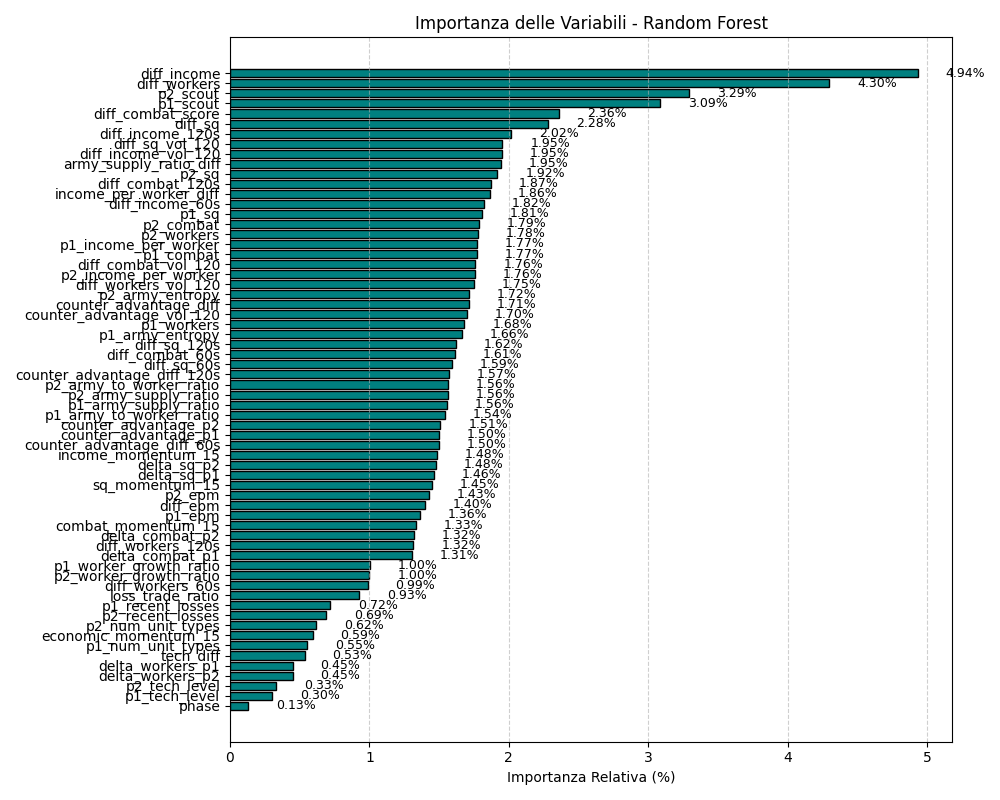
\includegraphics[width=0.88\textwidth]{rf_feature_importance.png}
    \caption{Stable top RF features across seeds. The strongest RF model relies primarily on broad game-state signals rather than explicit counter heuristics.}
    \label{fig:rfstable}
\end{figure}

This finding is methodologically important because it links the profile study to model interpretation: removing counter features did not simply simplify the model, it also aligned the RF winner with the feature families that repeatedly carry the strongest stable signal.

\subsection{Final full benchmark}
The core final benchmark consists of:
\begin{itemize}
    \item 2 model families (RF and XGB),
    \item 2 final dataset variants (\texttt{v3\_1\_fixed} and \texttt{v3\_2\_combatfix}),
    \item 3 replay-aware seeds (42, 43, 44).
\end{itemize}

This yields 12 full final tabular runs. These runs are the main source of the final scientific conclusions. Their purpose is not only to identify the best numerical score, but to determine which claims are stable enough to survive the jump from staged evidence to full-data evidence. In particular, the full benchmark answers three questions simultaneously:
\begin{enumerate}
    \item Does RF still benefit from the \texttt{no\_counter} profile at final scale?
    \item Does XGB still preserve its probability-quality advantage once evaluated under the same split discipline?
    \item Does \texttt{v3\_2\_combatfix} remain stronger than \texttt{v3\_1\_fixed}, or was that only an intermediate staged impression?
\end{enumerate}

\subsection{Deep challenger}
The deep branch is intentionally placed after the tabular finalists stabilize. Its job is not to define the benchmark prematurely, but to test whether a tuned MLP can overtake the two strongest tabular pipelines under the same full-data discipline. The deep branch is evaluated on \texttt{v3\_1\_fixed}, which survives the dataset-version comparison as at least as strong as \texttt{v3\_2\_combatfix}.

The deep experiment therefore functions as a strong challenger rather than as an exploratory curiosity. It asks whether a flexible non-linear learner, given the same replay-aware protocol and a controlled model-selection procedure, can produce a better final result than the tabular ensembles. This keeps the project from overcommitting too early to trees alone.

\subsection{Calibration experiment}
The calibration experiment is a final-layer experiment rather than an auxiliary appendix. Once the finalists are fixed, each finalist is re-evaluated through a stricter probability-quality lens. Validation predictions are used to fit post-hoc mappings, and test predictions remain untouched until the final calibrated evaluation. The purpose is to determine whether the finalist that looks strongest on log loss is also the finalist with the most trustworthy probabilities after held-out calibration is taken into account.


\section{Results}
\subsection{Final full multi-seed comparison}
The final full multi-seed benchmark compares RF and XGB on both dataset variants. Table~\ref{tab:finalmain} reports the mean and standard deviation over seeds 42, 43, and 44.

\begin{table}[H]
\centering
\caption{Final full multi-seed benchmark. Mean $\pm$ standard deviation over seeds 42, 43, and 44.}
\label{tab:finalmain}
\small
\resizebox{\textwidth}{!}{%
\begin{tabular}{l l l c c c c}
\toprule
Dataset & Model & Profile & Accuracy & Bal. Acc. & ROC-AUC & Log Loss \\
\midrule
\texttt{v3\_1\_fixed} & RF  & \texttt{no\_counter} & 0.6133 $\pm$ 0.0055 & 0.6111 $\pm$ 0.0051 & 0.6605 $\pm$ 0.0055 & 0.6503 $\pm$ 0.0023 \\
\texttt{v3\_1\_fixed} & XGB & \texttt{full}        & 0.6128 $\pm$ 0.0054 & 0.6093 $\pm$ 0.0049 & 0.6601 $\pm$ 0.0048 & 0.6484 $\pm$ 0.0025 \\
\texttt{v3\_2\_combatfix} & RF  & \texttt{no\_counter} & 0.6128 $\pm$ 0.0052 & 0.6107 $\pm$ 0.0048 & 0.6603 $\pm$ 0.0057 & 0.6504 $\pm$ 0.0024 \\
\texttt{v3\_2\_combatfix} & XGB & \texttt{full}        & 0.6128 $\pm$ 0.0069 & 0.6093 $\pm$ 0.0062 & 0.6597 $\pm$ 0.0059 & 0.6486 $\pm$ 0.0030 \\
\bottomrule
\end{tabular}%
}
\normalsize
\end{table}

\begin{figure}[H]
\centering
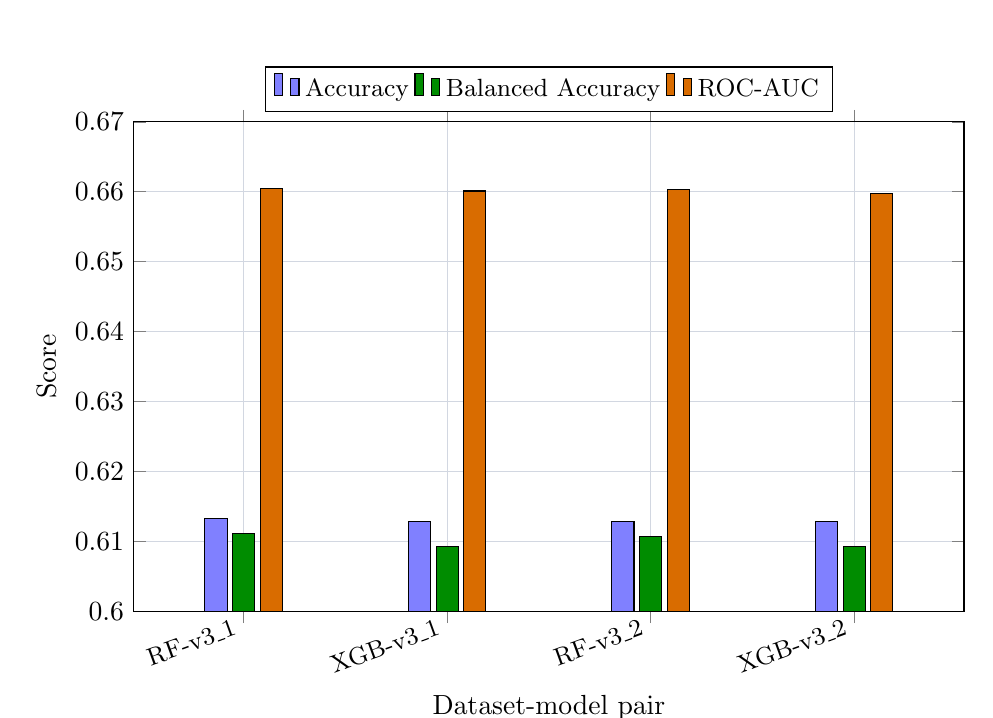
\begin{tikzpicture}
\begin{axis}[
width=\textwidth,
height=7.8cm,
ybar,
bar width=8pt,
xlabel={Dataset-model pair},
ylabel={Score},
symbolic x coords={RF-v3\_1,XGB-v3\_1,RF-v3\_2,XGB-v3\_2},
xtick=data,
xticklabel style={rotate=20,anchor=east,font=\small},
legend style={at={(0.5,1.02)},anchor=south,legend columns=4,font=\small},
ymin=0.60,ymax=0.67,
grid=major,
grid style={draw=linegray},
enlarge x limits=0.18
]
\addplot[fill=blue!50] coordinates {(RF-v3\_1,0.6133) (XGB-v3\_1,0.6128) (RF-v3\_2,0.6128) (XGB-v3\_2,0.6128)};
\addplot[fill=green!55!black] coordinates {(RF-v3\_1,0.6111) (XGB-v3\_1,0.6093) (RF-v3\_2,0.6107) (XGB-v3\_2,0.6093)};
\addplot[fill=orange!85!black] coordinates {(RF-v3\_1,0.6605) (XGB-v3\_1,0.6601) (RF-v3\_2,0.6603) (XGB-v3\_2,0.6597)};
\legend{Accuracy,Balanced Accuracy,ROC-AUC}
\end{axis}
\end{tikzpicture}
\caption{Classification-oriented view of the final full multi-seed comparison. RF and XGB remain extremely close on both dataset variants.}
\label{fig:fullcompare}
\end{figure}

Two conclusions are stable.
\begin{enumerate}
    \item \texttt{v3\_1\_fixed} is at least as strong as \texttt{v3\_2\_combatfix} at final scale. The staged suggestion that \texttt{v3\_2\_combatfix} might dominate does not survive the full benchmark.
    \item RF and XGB remain practically very close at project end-state, but with a clean trade-off: RF is marginally stronger on classification-oriented metrics, while XGB is marginally stronger on log loss.
\end{enumerate}

\subsection{Model-family interpretation}
The near-tie is not a weakness of the project; it is one of its most important outcomes. Earlier staged experiments gave the impression that the benchmark might collapse to a simple hierarchy, especially in favor of XGB and, in some regimes, in favor of \texttt{v3\_2\_combatfix}. The full benchmark shows that the problem is more subtle. Once the full replay-aware multi-seed evidence is considered, RF and XGB remain so close that the final recommendation must depend on the downstream objective rather than on a simplistic single-winner narrative.

This is exactly where the distinction between metric families becomes essential. RF leads very slightly on accuracy, balanced accuracy, and ROC-AUC. XGB leads very slightly on log loss and later also remains stronger in the probability-quality analysis. In other words, the project does not conclude that one model uniformly dominates the other. It concludes that the two models occupy different points on the same final Pareto-like front: one classification-oriented, one probability-oriented.

No formal significance test is reported for the final RF--XGB gap. The practical interpretation is therefore intentionally conservative: the final benchmark supports a small and stable trade-off between the two finalists, rather than evidence for a statistically decisive overall winner.

\subsection{Dataset-version interpretation}
The dataset-version result is equally important. During the staged phase, \texttt{v3\_2\_combatfix} appeared promising and sometimes looked stronger. The full benchmark changes that interpretation. At final scale, \texttt{v3\_1\_fixed} is at least as strong as \texttt{v3\_2\_combatfix}, and in some comparisons marginally stronger. This does not mean that the combat-fix idea was useless. It means that the final benchmark did not support a strong enough gain to justify rewriting the project conclusion around it.

Methodologically, this is one of the strongest results of the paper: the project does not simply report the most optimistic intermediate trend. It waits for the highest-quality evidence and then updates the story when the earlier trend does not hold strongly enough.

\subsection{Why the tie matters}
Scientifically, the near-tie is therefore meaningful. It shows that the strongest final conclusion is not ``XGB wins'' or ``RF wins'', but rather:
\begin{itemize}
    \item \textbf{RF + \texttt{v3\_1\_fixed} + \texttt{no\_counter}} is the strongest classification-oriented recommendation.
    \item \textbf{XGB + \texttt{v3\_1\_fixed} + full features} is the strongest probability-oriented recommendation.
\end{itemize}

This is a more nuanced conclusion than the staged story, but also a more honest one. It preserves the best parts of both finalists rather than overclaiming a narrow numerical edge as if it were a categorical victory.

\subsection{Temporal behavior}
The project also examined whether prediction quality shifts across different match durations. The temporal curves are not the basis of the final model choice, but they provide an additional sanity check that the predictive task behaves smoothly rather than being dominated by a narrow duration band.

\begin{figure}[H]
\centering
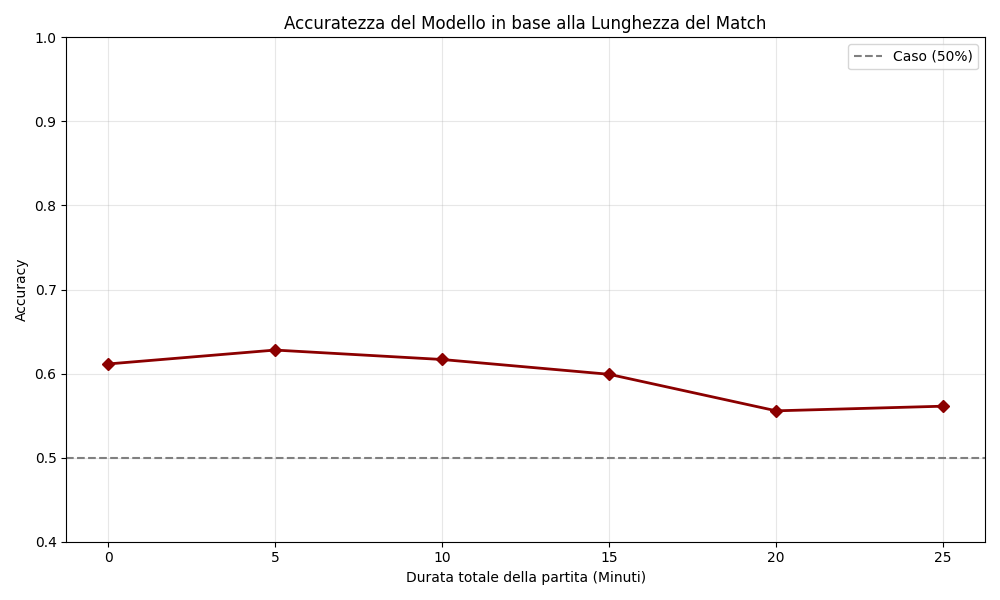
\includegraphics[width=0.48\textwidth]{accuracy_vs_duration.png}\hfill
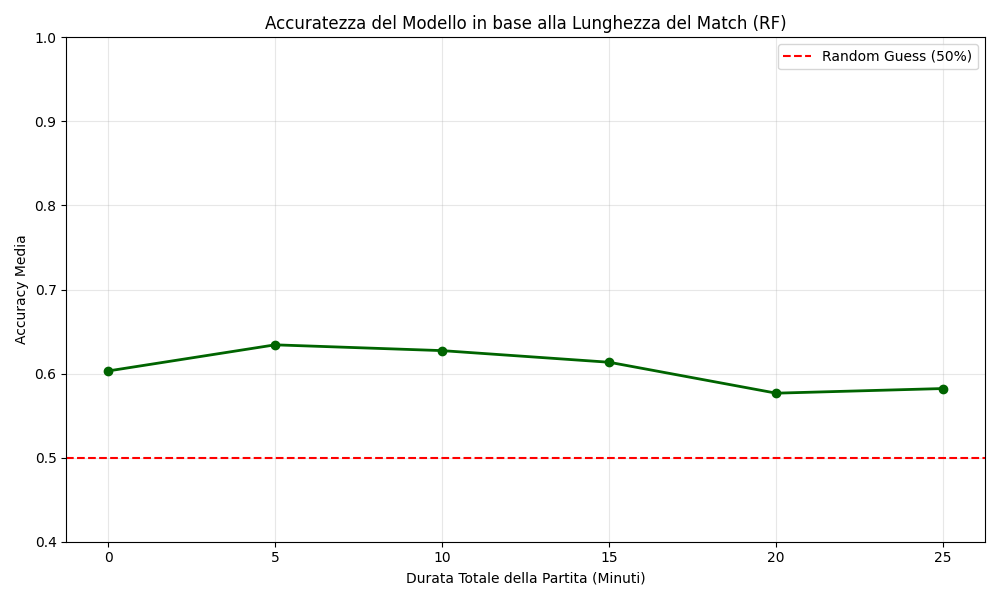
\includegraphics[width=0.48\textwidth]{rf_accuracy_vs_duration.png}
\caption{Temporal behavior of prediction accuracy. Left: overall accuracy vs. match duration. Right: RF-specific accuracy vs. duration.}
\label{fig:duration}
\end{figure}


\section{Calibration}
Calibration was treated as a proper validation-to-test procedure rather than as a descriptive add-on. For each finalist and seed, the model first produced validation predictions and test predictions. Two post-hoc calibrators were then fit on validation only:
\begin{itemize}
    \item Platt scaling,
    \item isotonic regression.
\end{itemize}
The learned mappings were finally applied to the untouched test predictions. This protocol matters because calibration can otherwise be made artificially optimistic by leaking information from the final test split into the probability mapping itself. In other words, the calibration step was evaluated under the same held-out discipline as the classifier comparison.

Table~\ref{tab:calibration} summarizes the aggregated calibration comparison on \texttt{v3\_1\_fixed}. The table is especially useful because it distinguishes two very different probability behaviors. RF starts from a probability output that is already competitive, but still noticeably benefits from post-hoc correction. XGB, by contrast, is already strong in uncalibrated form, and the post-hoc transforms do not produce a meaningful additional gain.

\begin{table}[H]
\centering
\caption{Rigorous calibration summary on \texttt{v3\_1\_fixed}. Lower is better for Brier, ECE, and MCE.}
\label{tab:calibration}
\begin{tabularx}{\textwidth}{l l c c c c}
\toprule
Model & Calibration & Accuracy & Brier & ECE(15) & MCE(15) \\
\midrule
RF \texttt{no\_counter} & uncalibrated & 0.612270 & 0.230209 & 0.025268 & 0.086660 \\
RF \texttt{no\_counter} & Platt        & 0.612597 & 0.229506 & 0.014375 & 0.052273 \\
RF \texttt{no\_counter} & isotonic     & 0.611708 & 0.229527 & 0.013742 & 0.040328 \\
XGB \texttt{full}       & uncalibrated & 0.612792 & 0.228850 & 0.013129 & 0.031368 \\
XGB \texttt{full}       & Platt        & 0.612788 & 0.228928 & 0.014968 & 0.072653 \\
XGB \texttt{full}       & isotonic     & 0.612098 & 0.228977 & 0.014071 & 0.044515 \\
\bottomrule
\end{tabularx}
\end{table}

\begin{figure}[H]
\centering
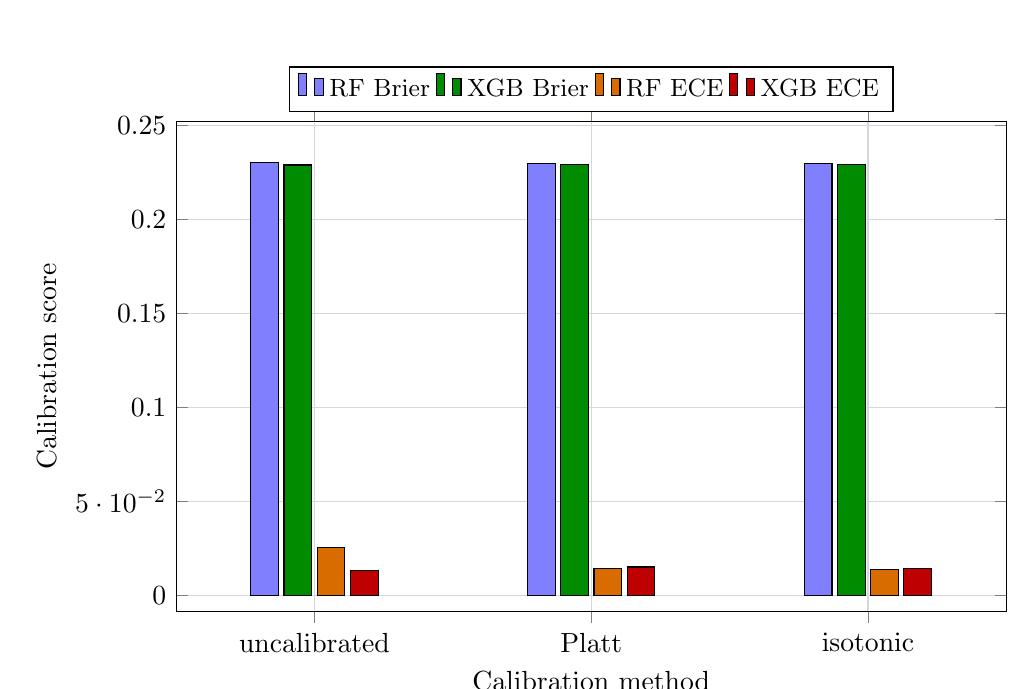
\begin{tikzpicture}
\begin{axis}[
width=\textwidth,
height=7.8cm,
ybar,
bar width=10pt,
xlabel={Calibration method},
ylabel={Calibration score},
symbolic x coords={uncalibrated,Platt,isotonic},
xtick=data,
legend style={at={(0.5,1.02)},anchor=south,legend columns=4,font=\small},
grid=major,
grid style={draw=linegray},
enlarge x limits=0.25
]
\addplot[fill=blue!50] coordinates {(uncalibrated,0.230209) (Platt,0.229506) (isotonic,0.229527)};
\addplot[fill=green!55!black] coordinates {(uncalibrated,0.228850) (Platt,0.228928) (isotonic,0.228977)};
\addplot[fill=orange!85!black] coordinates {(uncalibrated,0.025268) (Platt,0.014375) (isotonic,0.013742)};
\addplot[fill=red!75!black] coordinates {(uncalibrated,0.013129) (Platt,0.014968) (isotonic,0.014071)};
\legend{RF Brier,XGB Brier,RF ECE,XGB ECE}
\end{axis}
\end{tikzpicture}
\captionsetup{width=0.9\textwidth}
\caption{Calibration comparison. RF benefits substantially from post-hoc calibration, whereas XGB is already strong in uncalibrated form. Lower is better.}
\label{fig:calibration}
\end{figure}

The calibration conclusion is therefore very clear:
\begin{itemize}
    \item RF benefits noticeably from post-hoc calibration;
    \item XGB is already well calibrated in uncalibrated form;
    \item XGB remains the most defensible probability-oriented choice even after calibration is considered.
\end{itemize}

This calibration result sharpens the main project trade-off. RF remains attractive when the downstream objective is hard winner prediction and one is willing to calibrate the probabilities afterward. XGB, however, is the cleaner probability model because its raw probabilities are already stable and well behaved, which makes it the stronger candidate when probability estimates themselves are part of the downstream decision process.

\section{Deep Challenger}
The deep challenger was evaluated on full \texttt{v3\_1\_fixed} under the same replay-aware full-scale discipline used for the tabular finalists. It was included not as a toy baseline, but as a serious test of whether a flexible neural model could exploit non-linear interactions beyond what RF and XGB already captured. Candidate selection was performed on validation using a controlled family of MLP configurations that varied profile, scaler, activation, and architecture. This design gave the deep branch a fair opportunity to compete while keeping the search space narrow enough to remain interpretable and reproducible.

The final deep result is summarized in Table~\ref{tab:deep}.

\begin{table}[H]
\centering
\caption{Deep finalist result on full \texttt{v3\_1\_fixed}. Mean $\pm$ standard deviation over seeds 42, 43, and 44.}
\label{tab:deep}
\small
\setlength{\tabcolsep}{4pt}
\resizebox{\textwidth}{!}{%
\begin{tabular}{l l l c c c c}
\toprule
Dataset & Model & Profile & Accuracy & Bal. Acc. & ROC-AUC & Log Loss \\
\midrule
\texttt{v3\_1\_fixed} & Deep finalist & best candidate per seed & 0.6093 $\pm$ 0.0051 & 0.6083 $\pm$ 0.0042 & 0.6581 $\pm$ 0.0041 & 0.6506 $\pm$ 0.0025 \\
\bottomrule
\end{tabular}%
}
\normalsize
\end{table}

Because Accuracy and ROC-AUC are higher-is-better while Log Loss is lower-is-better, the deep comparison is summarized primarily through Table~\ref{tab:deep} rather than through a mixed-direction aggregate figure. This keeps the interpretation aligned with the metric semantics and avoids overcompressing the comparison into a single visual axis.


The deep branch is therefore not a failed branch. It reaches the same performance neighborhood as RF and XGB, which is itself a useful result because it shows that the replay-snapshot dataset contains enough structure for a reasonably tuned neural tabular model to remain competitive. However, it remains slightly below both tabular finalists, so its correct role in the project is \emph{credible challenger} rather than \emph{final winner}. In the final interpretation of the project, the deep result strengthens the confidence that the tabular finalists were not merely the winners by default; they remained the strongest models even after a serious neural challenger was tested under the same held-out discipline.

\section{Conclusions}
The final project conclusions are more nuanced, and more scientifically trustworthy, than the conclusions suggested by earlier staged runs. A major contribution of the project is not just the final leaderboard, but the way in which that leaderboard was stress-tested across dataset variants, replay-aware seeds, feature-profile changes, probability calibration, and a final deep challenger.

\begin{resultbox}
The project ends with two defensible finalists rather than one dominant winner.
\end{resultbox}

The stable conclusions are:
\begin{enumerate}
    \item \texttt{v3\_1\_fixed} remains at least as strong as \texttt{v3\_2\_combatfix} at final scale.
    \item RF and XGB are practically very close in the final full multi-seed comparison.
    \item RF with profile \texttt{no\_counter} is marginally stronger on classification-oriented metrics.
    \item XGB with the full feature set is marginally stronger on probability-oriented metrics and remains well calibrated without meaningful post-hoc gains.
    \item The deep challenger is competitive but does not surpass the tabular finalists.
\end{enumerate}

This leads to two final recommendations.
\begin{itemize}
    \item If the priority is \textbf{classification}, the recommended final model is \textbf{RF + \texttt{v3\_1\_fixed} + \texttt{no\_counter}}.
    \item If the priority is \textbf{probability quality}, the recommended final model is \textbf{XGB + \texttt{v3\_1\_fixed} + full features}.
\end{itemize}

\section*{Acknowledged Limitations}
The project is strong as a reproducible tabular benchmark, but several limitations remain:
\begin{itemize}
    \item the winning models consume independent snapshot rows rather than explicit temporal sequences;
    \item the full experiments use engineered replay features rather than raw spatial tensors;
    \item the POMDP interpretation remains conceptual rather than an explicit solved sequential control model.
\end{itemize}

These limitations suggest future extensions toward sequence models, latent-state estimation, and policy-support systems rather than only static outcome prediction.

Overall, the final evidence supports the following interpretation. If the goal is the strongest classification-oriented tabular model, the most defensible recommendation is RF + \texttt{v3\_1\_fixed} + \texttt{no\_counter}. If the goal is the strongest probability-oriented model, the most defensible recommendation is XGB + \texttt{v3\_1\_fixed} + full features. The project therefore closes not with a single absolute winner, but with a robust and interpretable trade-off between two finalists whose strengths are now clearly separated.

\appendix
\section{Appendix A: Selected Stable RF Features}
Table~\ref{tab:rffeatures} reports the top stable RF features from the feature-stability study.

\begin{table}[H]
\centering
\caption{Top stable RF features across seeds.}
\label{tab:rffeatures}
\begin{tabular}{lcc}
\toprule
Feature & Mean importance & Std. dev. \\
\midrule
\texttt{diff\_income} & 0.0373 & 0.0049 \\
\texttt{p2\_scout} & 0.0337 & 0.0008 \\
\texttt{p1\_scout} & 0.0326 & 0.0007 \\
\texttt{diff\_workers} & 0.0317 & 0.0061 \\
\texttt{diff\_combat\_score} & 0.0219 & 0.0018 \\
\texttt{diff\_sq\_vol\_120} & 0.0205 & 0.0014 \\
\texttt{diff\_sq} & 0.0204 & 0.0007 \\
\texttt{diff\_income\_vol\_120} & 0.0204 & 0.0009 \\
\bottomrule
\end{tabular}
\end{table}

\section{Appendix B: Reproduction Summary}
The final paper is supported by the following core artifacts in the project repository:
\begin{itemize}
    \item full multi-seed RF results on \texttt{v3\_1\_fixed} and \texttt{v3\_2\_combatfix};
    \item full multi-seed XGB results on \texttt{v3\_1\_fixed} and \texttt{v3\_2\_combatfix};
    \item full deep-finalist results on \texttt{v3\_1\_fixed};
    \item validation-to-test calibration artifacts for the final RF and XGB candidates.
\end{itemize}
Heavy datasets are stored as external zipped artifacts and are expected to be added to the final repository under the canonical paths used by the training scripts.

\section{Appendix C: SC2 Snapshot Formulation as a POMDP-like Model}
\label{app:pomdp}
Although the main study is framed as supervised learning over replay-derived snapshots, the underlying StarCraft II process is naturally partially observable. A snapshot cannot reveal the full latent strategic state of the match: hidden technology, private production intent, incomplete scouting, local tactical geometry, and future transitions remain only partially observed. For that reason, the snapshot-learning view used in this paper is compatible with a higher-level POMDP interpretation.

At a conceptual level, one may define a model
\[
\mathcal{M} = (S, A, O, T, Z, R, b_0),
\]
where $S$ is the latent strategic state space, $A$ is a set of high-level strategic actions, $O$ is the observation space induced by the replay features, $T$ is the latent transition model, $Z$ is the observation model, $R$ is a strategic reward signal, and $b_0$ is the initial belief. Under this interpretation, the engineered feature vector at time $t$ is not the true state itself but an observation
\[
o_t = \phi(s_t, \varepsilon_t),
\]
with $\varepsilon_t$ absorbing aggregation error, partial observability, and compression effects. The learned predictor can therefore be interpreted as operating on observation-level surrogates of belief-relevant information rather than on the full underlying game state.

This appendix is intentionally brief because the POMDP-like interpretation is a conceptual extension, not the main experimental contribution of the paper. A separate companion PDF in the project artifacts discusses the SC2 snapshot POMDP-like formulation in more detail, including the role of latent strategic state, observation compression, and belief-style approximations. In the present paper, the purpose of this appendix is only to clarify why static replay snapshots can still carry meaningful strategic signal while also motivating future work on sequence models, latent-state estimation, and decision-making under partial observability.

\end{document}
